
\subsection*{\textbf{Question 4.c}}
\begin{quote}

\textbf{Problem}
\begin{quote} 
Use the Zeldovich approximation to generate a movie of the evolution of a volume in two dimensions
from a scale factor of 0.0025 until a scale factor of 1.0. To do this, start with 64x64 particles arranged in a square grid with a grid spacing of 1 Mpc. Use $P(k) = k^{-2}$ and the given equation to generate $c_k$, then use the FFT on your grid of particles to calculate $\textbf{S(q)}$. As $a$ increases, update the positions and momenta of the particles and save each step as a frame for your movie. 
\end{quote}

\textbf{Solution} 
\begin{quote}
The difficulty in this exercise lays by determining the displacement vector. The displacement vector is calculated by first creating a matrix in $k-space$ with complex values based on the given power law. The matrix is next given the correct hermitian symmetry, (see exercise 2). The components of the displacement vector, $s_x$ and $s_y$, are then calculated independent with the help of this matrix.  This calculation is done as follows. First the hemitian matrix is multiplyed with the wavenumbers and $1i$ to obtain two matrices where the cells have respectively values of $ic_k k_x$ and $ic_k k_y$. After this multiplication the matrix cannot be directly fourier transformed to obtain $s_x$ and $s_y$, as the multiplication with the wavenumbers breaks the symmetry in the columns with nyquest wavenumbers. The symmetry is only broken by a minus sign and this is corrected before doing the IFFT. 
\\
The code that creates the movie and the plots can be found below. The final plot of the simulation is also included and shows that the particles clearly move to the denser region.

\end{quote}

\textbf{Code -plots}:
\begin{quote}

The code that creates the movie and the plots of the first 10 particles. 
\lstinputlisting[firstline = 27, lastline=158]{./Code/assigment_4.py}
\end{quote}

\textbf{Plots - field}

\begin{quote}
\begin{figure}[!ht]
\centering
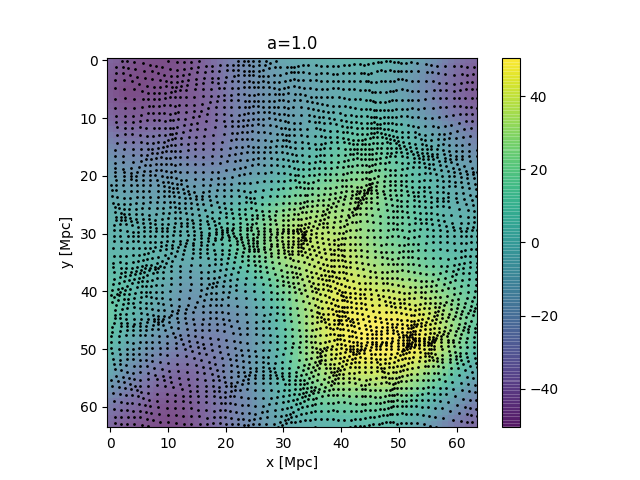
\includegraphics[width=14cm, height=9.5cm]{./Plots/4c/4c=89.png}
\caption{The final plot of the movie. It can clearly be seen that the particles (black dots) moved to the denser region. }
\label{FIG:stuff}
\end{figure}
\end{quote}
\newpage

\textbf{Plots - particles}
\begin{quote}
\begin{figure}[!ht]
\centering
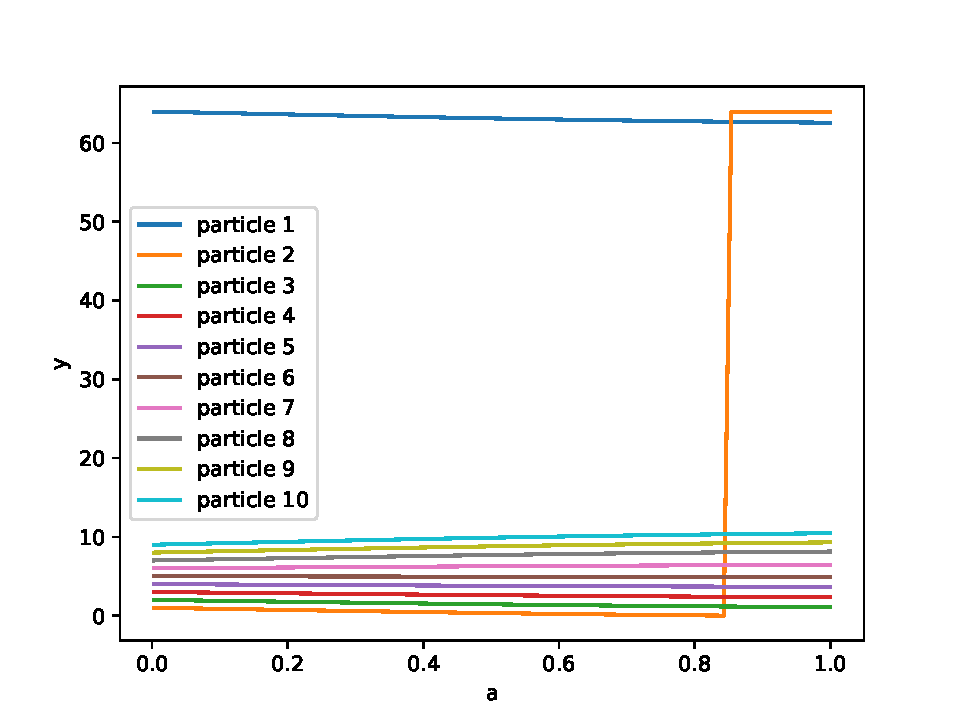
\includegraphics[width=14cm, height=8.5cm]{./Plots/4c_pos.pdf}
\caption{The y-positions of the first 10 particles. The plot shows that the particles are slowly moving to a denser region (see figure \ref{FIG:stuff}, where the first 10 particles are at the left top). The large jump for particle 2 (orange) at a scale factor of around $ a \approx 0.8$ is the result of the circular boundary conditions.  }
\end{figure}
\begin{figure}[!ht]
\centering
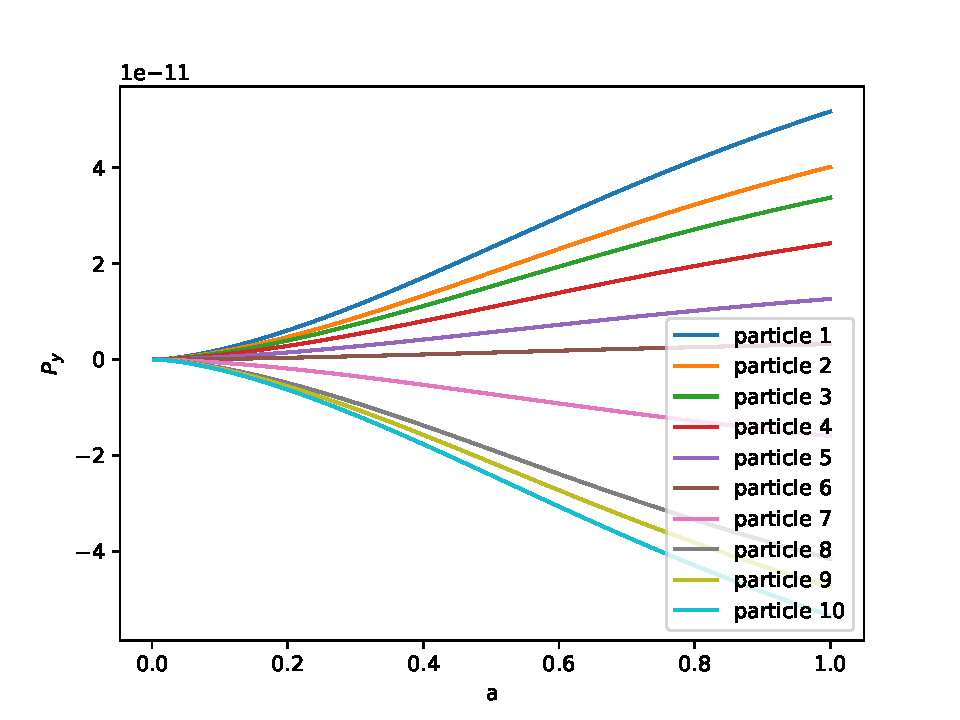
\includegraphics[width=14cm, height=8.5cm]{./Plots/4c_momentum.pdf}
\caption{The momentum of the first 10 particles. The fact that about halve of the particles have a positive momentum and that the other halve have a negative momentum is a result of the circular boundary conditions and the created field.  }
\end{figure}
\end{quote}
\newpage


\end{quote}




